\documentclass[10pt]{article}
\usepackage[a4paper,margin=18mm]{geometry}
\usepackage[T1]{fontenc}\usepackage{lmodern}
\usepackage{amsmath,amssymb,booktabs,array,enumitem}
\usepackage{tikz}\usetikzlibrary{shapes.gates.logic.US,positioning,arrows.meta}
\usepackage[hidelinks]{hyperref}
\setlength{\parindent}{0pt}\setlength{\parskip}{4pt}\setlength{\emergencystretch}{2em}
\newcommand{\mos}[4]{\begin{scope}[shift={(#1,#2)}]
\draw(0,.24)--(0,-.24);\draw(0,.2)--(.25,.2)--(.25,.5);\draw(0,-.2)--(.25,-.2)--(.25,-.5);
\draw(-.16,.23)--(-.16,-.23);
\ifnum#4=1\draw(-.26,0)circle(.06);\draw(-.75,0)--(-.32,0);\else\draw(-.75,0)--(-.16,0);\fi
\node[anchor=east,font=\scriptsize]at(-.76,0){$#3$};\end{scope}}
\newcommand{\gnd}[2]{\draw(#1,#2)--(#1,{#2-.12});\draw({#1-.17},{#2-.12})--({#1+.17},{#2-.12});\draw({#1-.11},{#2-.2})--({#1+.11},{#2-.2});}
\newcommand{\rail}[3]{\draw(#1,#2)--(#1,{#2+.14});\node[above,font=\scriptsize]at(#1,{#2+.14}){$#3$};}
\begin{document}
\begin{center}\large\textbf{EE3032 Introduction to VLSI -- Midterm}\\\normalsize Fall 2022 -- reconstructed original paper, 100 points\end{center}
\textit{The complete original printed pages 2-1 and 2-2 are available. Text, numbering, marks and circuit connections are retained; handwritten annotations are not exam constraints.}\par
\textbf{1. (35 points)} Answer the following questions briefly.
\begin{enumerate}[label=(\alph*),leftmargin=7mm,itemsep=3pt]
\item List the process for transferring the mask pattern to the surface of a silicon region. (3 points)
\item What is silicon on insulator process? Explain how it can reduce the leakage current. (4 points)
\item List two methods for the oxidation in silicon. (2 points)
\item List two features of static CMOS circuits. (2 points)
\item List two components of CMOS circuit, which can result in static power. (2 points)
\item In a logic gate, we usually implement the pull-up network with PMOS transistors and the pull-down network with NMOS transistors. Why? (2 points)
\item One of modern CMOS process technologies provides high-k and metal gate transistor. Explain why the high-k material is used. (2 points)
\item List two through-silicon via (TSV) process technologies. (2 points)
\item In a CMOS gate, the transistors connected to the gate output suffer from the severe body effect. Why? (2 points)
\item What is antenna effect? List two design methods for the fixing of antenna effect violation. (6 points)
\item List three bonding technologies for 3D ICs. (3 points)
\item The output capacitance of a CMOS logic gate in a CMOS circuit is comprised of three components. List the three components. (3 points)
\item List two types of FinFET structures. (2 points)
\end{enumerate}\newpage\textbf{2. (20 points)} Fig. 1(a) shows the block diagram of an 8-to-1 multiplexer.
\begin{enumerate}[label=(\alph*),leftmargin=7mm]
\item Design the multiplexer using transmission gate. (10 points)
\item What is the relationship of the multiplexer delay to the number of selection inputs $(s_0s_1s_2)$. Explain your answer. (5 points)
\item Assume that the circuit shown in Fig. 1(b) realizes the function $F=AB+\overline{B}C+D$. Complete the circuit. (5 points)
\end{enumerate}\begin{center}\begin{tikzpicture}[font=\small]
\draw(-.5,.8)--(-.5,-.8)--(.3,-.45)--(.3,.45)--cycle;
\draw(-.5,.55)--(-1.1,.55)node[left]{$x_0$};\draw(-.5,.25)--(-1.1,.25)node[left]{$x_1$};
\node at(-.85,-.05){$\vdots$};\draw(-.5,-.55)--(-1.1,-.55)node[left]{$x_7$};\draw(.3,0)--(.8,0)node[right]{$y$};
\foreach\x/\z/\s in {-.4/-.9/s_0,-.15/-.15/s_1,.1/.6/s_2}{\draw(\x,-.75)--(\x,-.95)--(\z,-1.15)node[below]{$\s$};}
\node at(-.2,-1.75){(a)};
\begin{scope}[shift={(4.5,0)}]
\draw(-.4,.8)--(-.4,1.6)--(.3,1.4)--(.3,1.0)--cycle;\node at(-.2,1.4){0};\node at(-.2,1){1};
\draw(-.4,-1.6)--(-.4,-.8)--(.3,-1.0)--(.3,-1.4)--cycle;\node at(-.2,-1){0};\node at(-.2,-1.4){1};
\draw(1.5,-.4)--(1.5,.4)--(2.2,.2)--(2.2,-.2)--cycle;\node at(1.7,.2){0};\node at(1.7,-.2){1};
\draw(.3,1.2)--(.8,1.2)|-(1.5,.2);\draw(.3,-1.2)--(.8,-1.2)|-(1.5,-.2);\draw(2.2,0)--(2.8,0)node[right]{$F$};
\foreach\y in {1.4,1,-1,-1.4}{\draw(-.4,\y)--(-.9,\y);}\draw(-.05,.9)--(-.05,.55);\draw(-.05,-1.5)--(-.05,-1.95);\draw(1.85,-.3)--(1.85,-1.95);
\node at(1,-2.25){(b)};\end{scope}
\end{tikzpicture}\\Figure 1: (a) 8-to-1 multiplexer. (b) Multiplexer-based circuit.\end{center}\textbf{3. (10 points)} Fig. 2(a) shows a CMOS circuit driving a large capacitance $C_L=2.98\,\mathrm{pF}$. For the used process, the input capacitance $C_g$ of a minimum-size inverter (i.e., the size of NMOS and PMOS is $W_{min}/L_{min}$) is $1\,\mathrm{fF}$. Assumptions: 1) the drain and wire parasitic capacitance can be neglected; 2) $e=2.7$, $e^4=55$, $e^6=403$, and $e^8=2980$; 3) $\mu_n=2\mu_p$; 4) the turn-on resistance of an NMOS transistor with $W_{min}/L_{min}$ is $R$.
\begin{enumerate}[label=(\alph*),leftmargin=7mm]
\item Design a super buffer as shown in Fig. 2(b) to drive the large capacitance such that the output load of the NAND gate A is $C_g$ and the delay $T$ is minimized. (5 points)
\item For the designed super buffer, if the size of NMOS transistors is fixed and we desire to tune the size of PMOS transistors such that the rise time and fall time of each inverter are equal, determine the size of PMOS transistors of the super buffer. Estimate the delay $T$ in terms of $R$ and $C_g$ if the modified super buffer is used! (5 points)
\end{enumerate}\begin{center}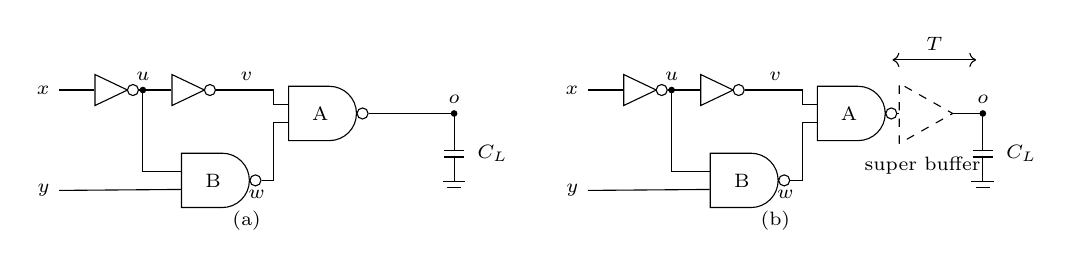
\begin{tikzpicture}[x=.85cm,y=.85cm,font=\scriptsize]\begin{scope}[shift={(0,0)}]
\node[not gate US,draw](i1)at(.6,1.7){};\node[not gate US,draw](i2)at(1.75,1.7){};
\draw(i1.input)--(-.1,1.7)node[left]{$x$};\draw(i1.output)--(i2.input);\node[above]at(1.15,1.7){$u$};
\node[nand gate US,draw,logic gate inputs=nn,logic gate input sep=.23cm](a)at(3.8,1.35){A};
\node[nand gate US,draw,logic gate inputs=nn,logic gate input sep=.23cm](b)at(2.2,.35){B};
\draw(i2.output)--(3.1,1.7)|-(a.input 1);\node[above]at(2.7,1.7){$v$};
\draw(1.15,1.7)--(1.15,.5)|-(b.input 1);\fill(1.15,1.7)circle(1.2pt);\draw(b.input 2)--(-.1,.2)node[left]{$y$};
\draw(b.output)--(3.1,.35)|-(a.input 2);\node[below]at(2.85,.35){$w$};
\draw(a.output)--(5.8,1.35);\node[above]at(5.8,1.35){$o$};\fill(5.8,1.35)circle(1.2pt);\draw(5.8,1.35)--(5.8,.8);\draw(5.65,.8)--(5.95,.8);\draw(5.65,.7)--(5.95,.7);\draw(5.8,.7)--(5.8,.45);\gnd{5.8}{.45};\node[right]at(6,.75){$C_L$};\node at(2.7,-.25){(a)};\end{scope}\begin{scope}[shift={(7.9,0)}]
\node[not gate US,draw](i1)at(.6,1.7){};\node[not gate US,draw](i2)at(1.75,1.7){};
\draw(i1.input)--(-.1,1.7)node[left]{$x$};\draw(i1.output)--(i2.input);\node[above]at(1.15,1.7){$u$};
\node[nand gate US,draw,logic gate inputs=nn,logic gate input sep=.23cm](a)at(3.8,1.35){A};
\node[nand gate US,draw,logic gate inputs=nn,logic gate input sep=.23cm](b)at(2.2,.35){B};
\draw(i2.output)--(3.1,1.7)|-(a.input 1);\node[above]at(2.7,1.7){$v$};
\draw(1.15,1.7)--(1.15,.5)|-(b.input 1);\fill(1.15,1.7)circle(1.2pt);\draw(b.input 2)--(-.1,.2)node[left]{$y$};
\draw(b.output)--(3.1,.35)|-(a.input 2);\node[below]at(2.85,.35){$w$};
\draw(a.output)--(4.55,1.35);\draw[dashed](4.55,.9)--(4.55,1.8)--(5.35,1.35)--cycle;\draw(5.35,1.35)--(5.8,1.35);\node[below,font=\scriptsize]at(4.9,.85){super buffer};\draw[<->](4.45,2.15)--(5.7,2.15)node[midway,above]{$T$};\node[above]at(5.8,1.35){$o$};\fill(5.8,1.35)circle(1.2pt);\draw(5.8,1.35)--(5.8,.8);\draw(5.65,.8)--(5.95,.8);\draw(5.65,.7)--(5.95,.7);\draw(5.8,.7)--(5.8,.45);\gnd{5.8}{.45};\node[right]at(6,.75){$C_L$};\node at(2.7,-.25){(b)};\end{scope}\end{tikzpicture}\\Figure 2: (a) A NAND gate driving a large capacitance. (b) A super buffer is inserted.\end{center}\newpage\textbf{4. (15 points)} Fig. 3(a) shows a CMOS logic gate. Assume that the threshold voltage of the NMOS transistor is $0.4\,\mathrm V$; the turn on resistance of N1, N2, and N3 is $R$, $2R$, and $R$, respectively.
\begin{enumerate}[label=(\alph*),leftmargin=7mm]
\item If the initial voltage of the output $V_{out}$ is $1.2\,\mathrm V$ and an input stimulus $(0\to1.2\,\mathrm V)$ as shown in Fig. 3(b) is applied, how much voltage of the input stimulus $(V_{in})$ at $x$ is? (9 points)
\item Identify the operation region of the transistors N1, N2, and N3 from $t_1$ to $t_2$. (6 points)
\end{enumerate}\begin{center}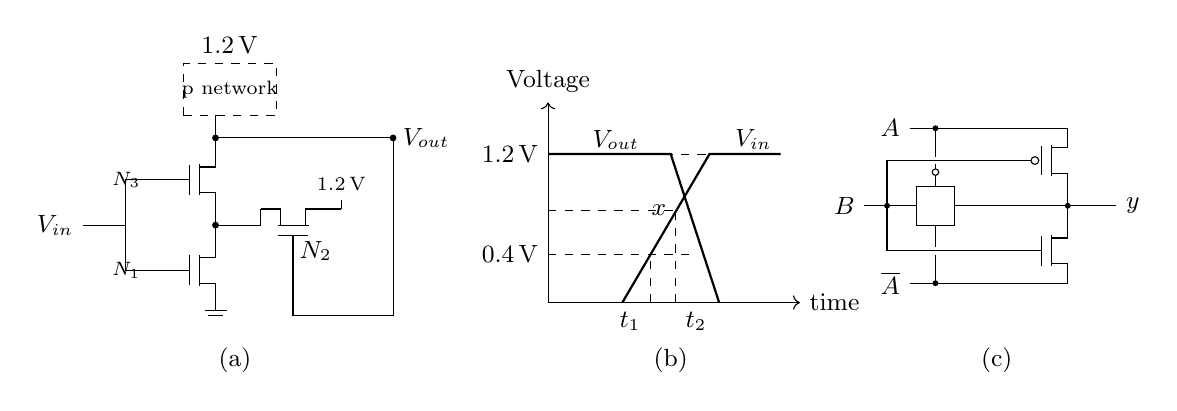
\begin{tikzpicture}[scale=.82,font=\small]
\draw[dashed](-.25,3.5)rectangle(1.2,4.3);\node[font=\scriptsize]at(.47,3.9){p network};\node[above]at(.47,4.3){$1.2\,\mathrm V$};
\draw(.25,3.5)--(.25,3.0);\mos{0}{2.5}{N_3}{0}\mos{0}{1.1}{N_1}{0}
\draw(.25,2)--(.25,1.6);\gnd{.25}{.6}
\draw(-.75,2.5)--(-1.15,2.5)--(-1.15,1.1)--(-.75,1.1);\draw(-1.15,1.8)--(-1.8,1.8)node[left]{$V_{in}$};
\draw(.25,3.15)--(3,3.15)node[right]{$V_{out}$};\fill(.25,3.15)circle(1.5pt);
\begin{scope}[shift={(1.45,1.8)},rotate=90]\mos{0}{0}{}{0}\end{scope}
\draw(.25,1.8)--(.95,1.8)--(.95,2.05);\fill(.25,1.8)circle(1.5pt);
\draw(1.95,2.05)--(2.2,2.05);\rail{2.2}{2.05}{1.2\,\mathrm V};\node at(1.8,1.4){$N_2$};
\draw(1.45,1.05)--(1.45,.4)--(3,.4)--(3,3.15);\fill(3,3.15)circle(1.5pt);
\begin{scope}[xshift=1.4cm]
\draw[->](4.0,.6)--(7.9,.6)node[right]{time};\draw[->](4,.6)--(4,3.7)node[above]{Voltage};
\draw[dashed](4,2.9)--(6.9,2.9);\node[left]at(4,2.9){$1.2\,\mathrm V$};
\draw[dashed](4,1.35)--(6.2,1.35);\node[left]at(4,1.35){$0.4\,\mathrm V$};
\draw[thick](4,2.9)--(5.9,2.9)--(6.65,.6);\node at(5.05,3.12){$V_{out}$};
\draw[thick](5.15,.6)--(6.5,2.9)--(7.6,2.9);\node at(7.18,3.13){$V_{in}$};
\draw[dashed](5.58,.6)--(5.58,1.35);\draw[dashed](5.98,.6)--(5.98,2.03);\node[below left]at(5.58,.6){$t_1$};\node[below right]at(5.98,.6){$t_2$};
\draw[dashed](4,2.03)--(5.98,2.03);\node[left]at(5.98,2.03){$x$};
\node at(5.9,-.3){(b)};\end{scope}\node at(.55,-.3){(a)};
\begin{scope}[shift={(11.2,.3)}]
\draw(-.2,3)--(2.25,3);\node[left]at(-.2,3){$A$};\draw(-.2,.6)--(2.25,.6);\node[left]at(-.2,.6){$\overline A$};
\mos{2}{2.5}{}{1}\mos{2}{1.1}{}{0}\draw(2.25,2)--(2.25,1.6);\draw(2.25,1.8)--(3,1.8)node[right]{$y$};\fill(2.25,1.8)circle(1.3pt);
\draw(-.1,1.5)rectangle(.5,2.1);\draw(.2,2.1)--(.2,2.27);\draw(.2,2.32)circle(.05);\draw(.2,2.37)--(.2,2.44);\draw(.2,2.56)--(.2,3);\fill(.2,3)circle(1.3pt);
\draw(.2,1.5)--(.2,1.16);\draw(.2,1.04)--(.2,.6);\fill(.2,.6)circle(1.3pt);
\draw(.5,1.8)--(2.25,1.8);\draw(-.9,1.8)--(-.1,1.8)node[pos=0,left]{$B$};\fill(-.55,1.8)circle(1.3pt);
\draw(-.55,1.8)--(-.55,2.5)--(1.25,2.5);\draw(-.55,1.8)--(-.55,1.1)--(1.25,1.1);
\node at(1.15,-.6){(c)};
\end{scope}\end{tikzpicture}\\Figure 3: (a) A CMOS logic gate. (b) Waveforms of $V_{in}$ and $V_{out}$. (c) A CMOS circuit.\end{center}\textbf{5. (10 points)} What function does the circuit shown in Fig. 3(c) realize? Does it have any weaknesses?\par\vspace{5mm}\textbf{6. (10 points)} Complete the following questions.
\begin{enumerate}[label=(\alph*),leftmargin=7mm]
\item Implement the following Boolean function: $F=X(Y+Z)+XW$ using CMOS logic. Draw the schematic diagram. (5 points)
\item We have a CMOS logic gate realizing $F=\overline{X(Y+Z)}$ and the sizes of all the NMOS and PMOS transistors of the CMOS logic gate are $W/L$. Design an equivalent inverter for analyzing the rise time $(t_r)$ and fall time $(t_f)$ of the logic gate with input transitions $XYZ:\ 101\to100\to101$. (5 points)
\end{enumerate}\end{document}